\section{Robothandens principiella funktion}
Robothanden följer användarens fingerrörelser tills dess att den greppar ett av flera fördefinerade, kända objekt, då den istället verkar för att hålla objektet med en önskad kraft, tills dess att användaren visar att den vill släppa objektet igen genom att öppna sin hand. Nedan visas ett flödesschema för överskådligt beskriva hur robothanden principiellt fungerar.
\begin{figure}[H]
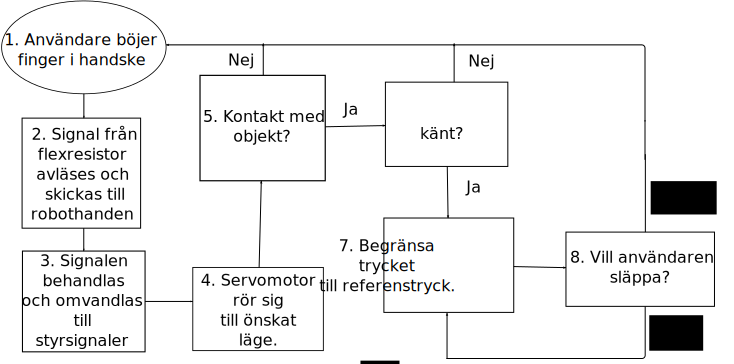
\includegraphics[width=.90\textwidth]{img/flodesschema}
\caption{Flödesschema över en tänkt signals väg genom robothanden.}
\end{figure}
\begin{enumerate}
\item Önskat fingerläge ges genom att användaren böjer sitt finger i kontrollhandsken. 
\item Flexresistor på kontrollhandsken ändrar resistans. 
\item Den ändrade resistansen avläses av en Arduino Micro enhet på kontrollhandsken som skickar den via bluetooth till en Arduino Mega enhet på robothanden.
\item Värdet på resistansen omvandlas till PWM-signal som kalibrerats av användaren vid uppstart BLÖBLÖBLÖBLBÖLBÖLBÖLBÖLB FORTSÄTT HÄR!!! 
\item PWM-signaler matas till aktuatorer som ställer sig i önskad vinkel. 
\item Feedback från trycksensorer avläses och leder till ett stopp av aktueringen om avläst tryck är högre än fördefinerad gräns.
\end{enumerate}
Robothanden kan delas in i tre delsystem som samverkar för att uppfylla handens funktion. Delsystemen är styrhandske, styrsystem och robothand. Användaren har på sig styrhandsken och styrsystemet verkar för att robothanden ska imitera användarens fingerrörelser tills dess att robothanden kommer i kontakt med ett objekt. 
\section{Robothanden}
FÖRKLARA FRIHETSGRADER?
I detta avsnitt presenteras en överblick över de komponenter som utgör den mekaniska handen.För spara tid har Meccano™ använts som grund vilket har både fördelar och nackdelar jämfört med att bygga alla delar från början. Eftersom konstruktionen innehåller flera delar vars inbördes passform påverkar hur väl rörelser fungerar måste tillverkningen av delarna utföras med god noggrannhet. Meccanos standardbyggsats innehåller flera olika standardiserade delar som enkelt kan monteras i flera olika kombinationer.Delarna anses även ha tillräcklig noggrannhet för att slutprodukten ska kunna utföra de uppsatta målen. Eftersom konstruktionen av handen går snabbare med färdiga delar kan mer fokus läggas på den mer resurskrävande elektroniken. Nackdelen är att konstruktionen blir begränsad till att endast kunna tillverkas av tillgängliga komponenter, men detta kringgås med konstruktion av enstaka kritiska komponenter.
Handen består av två fingrar och en tumme som beskrivs utförligare i sina respektive avsnitt. På fingrar och tumme sitter det även plastskal som har som uppgift att skapa bättre greppytor. 

BILD PÅ UTPROVNING AV GREPP

Handens utformning är en funktion av hur fingrarna önskas vara positionerade relativt varandra och detta utprovades i CAD-miljö utefter förmågan att utföra de önskade greppen. Handen har även tillräckligt stor yta för att möjliggöra integrering av aktuatorer, kontrollenhet och strömförsörjning i en enda enhet. I figuren ovan syns från vänster till höger LBLANBLABLABLABNBLABA som är de MÅL BLA BLA BLA



\subsection{Fingrar och tumme}
Med utgångspunkten mänsklig motorik designades handens två identiska fingrar för att få ett människolikt rörelsemönster.
BILD Översiktsbild fingerdesign
Fingrarna har tre leder varav Led 1 och Led 2 är separat kontrollerbara. Led 3 är via ett stag tvångsstyrd av Led 2 för att imitera hur ett mänskligt finger beter sig när handen sluts. Jämfört med det mänskliga fingret saknas en frihetsgrad i Led 1 för vridning av fingret i sidled. En fördel med två separat kontrollerbara leder är att fingrarnas rörelseomfång och funktionella förmåga utökas.

BILD TUMME. Tummen har endast två separata frihetsgrader och sitter fast positionerad i handen för att kunna utföra ett pincettgrepp med finger 1. Detta är tillräckligt för att uppnå målen, men jämfört med den mänskliga tummen som kan möta samtliga fingertoppar är detta ett stelt utförande.
%\begin{minipage}[t]{0.5\textwidth}
%\begin{figure}[H]
%\includegraphics[width=0.57\textwidth]{img/rorelse1}
%\caption{En kontrollerbar frihetsgrad.}
%\end{figure}
%\end{minipage}
%\begin{minipage}[t]{0.5\textwidth}
%\begin{figure}[H]
%\includegraphics[width=0.5\textwidth]{img/rorelseomfang}
%\caption{Två kontrollerbara frihetsgrader.}
%\end{figure}
%\end{minipage}

\subsection{Fingertoppar och sensorer}
BILD PÅ SENSORER, FINGERTOPPAR MED GUMMI och sensor PÅ(sprängskiss) 
Fingertopparna är formgivna för att kunna ge ett bra pincettgrepp där sensorerna registrerar hur hårt objektet greppas. Sensorerna är av modell FSR-400 och kan registrera normaltryck i spannet ca 0.11-110 MPa genom att ändra resistans vid kompression. Värdet på resistansen avläses av handens mikrokontroller och jämförs med kalibrerade värden från tester ( SE APP KALIBRERING AV SENSORER) för att säkerställa att handen griper med rätt tryck. Över sensorn sitter ett !!!X!!! mm tjockt gummi för att skydda sensorns samt ge större friktion vid hantering av objekt. Nedre delen av fingertoppen fungerar som stöd vid grepp där kontakttrycket inte mäts.
\section{Aktuering}
Total har handen åtta frihetsgrader varav sex är separat aktuerbara. I detta avsnitt presenteras aktuatorer och kraftöverföring.
\subsection{Servon}
BILD PÅ SERVO
Aktuatorer för samtliga leder är Blue Bird BMS-660DMG+HS. Dessa servon valdes för att de uppfyllde kraven på vridmoment med god marginal (se APPENDIX A.HIYTF för dimensionerande beräkningar). Vid spänningen 6 Volt har de ett maximalt vridmoment på 1.42 Nm och en högsta rotationshastighet på 6.16 rad/s utan belastning. De har ett totalt rörelseomfång på 120 grader som är standard för hobbyservos. Servona regleras via PWM-signal och har intern positionsreglering. Detta gör att de alltid kommer arbeta för att nå ett önskat läge med och kommer återgå till detta läge efter en eventuell störning.

\subsection{Kraftöverföring}
BILD PÅ STAG, BILD PÅ SENA MED HJUL
Led 1 i samtliga fingrar aktueras via stag, vilket gör att de kan föras fram och tillbaka av respektive servo. För att aktuera Led 2 i samtliga fingrar används en sena. Senan utgörs av en fiskelina dimensionerad för en dragkraft på 330 N. Största dragkraften i senan uppstår då servo arbetar vid maximalt vridmoment och uppgår till 118 N med 12 mm servohorn. För att återföra 

\section{Reglerhandsken}
För att reglera robothanden intuitivt används en reglerhandske. På handsken sitter flexsensorer som följer användarens hand och ändrar resistans beroende på hur mycket de böjs. Denna resistansförändring använder man som insignal till mikrokontrollen (Läs mer i 2.5)    

Handsken är gjord av textil och flexsensorerna är insydda i små påsar som underlättar montering av sensorerna på handsken. (Se figur)
(Bild på handsken)  


\section{Mikrokontroller}
info om våra microcontroller. Bluetooth moduelerna och hur det programmerats samt hur det fungerar.
\section{Elektriska kretsar}
ELSCHEMA HANDSKE, ROBOTHAND
Dedssa kretsar har byggts och lötts på kretskort- 

\section{Algoritmer}
Här presenteras de styralgortimter som bestämmer hur handen beter sig när den följer användarens input samt identifierar och greppar objekt. 
\subsection{Objektidentifiering}
EN BILD SOM FÖRKLARAR DETTA, SAMT VILKA OBJEKT VI VALT ATT identifierar och hur vi gör det...
Antaganden: Servona står i önskat läge, det vill säga tidsfördröjningen som uppstår då servona skall vrida sig från godtycklig position till den önskade antags vara så liten vid normalt användande att den kan försummas. Då ingen mätning av servonas verkliga position görs, är den enda informationen om fingrarnas lägen det önskade servoläget. 

FIXA FLÖDESSSCHEMA OCH ETT ARDUINO PROGRAM Känner av tryck (över visst gränsvärde) på tumme och motstående finger->, lagrar användarens input läge då detta inträffar ( för att när användaren går utanför detta igen (öppnar sin hand) så skall handen återgår till att följa användaren) -> beräknar avståndet mellan sensorerna-> checkar av avståndet mot en lista av fördefinerade objekt som innehåller , storlek och önskat trycksensorvärde med en +/-tolerans för att inte handen ska stå och flippa som en tok för att uppnå EXAKT rätt värde-> TADAA!!-> när användaren öppnar sina fingrar utanför "kontaktläget" följer handen efter igen...
Mer teksti


